\documentclass[12pt]{article}
\usepackage[a4paper, margin=1in]{geometry}
\usepackage{enumitem}
\usepackage{hyperref}
\usepackage{listings}
\usepackage{xcolor}
\usepackage{graphicx}
\usepackage{tikz}
\usepackage{amsmath}
\usepackage{amssymb}
\usepackage{booktabs}
\usepackage{multirow}
\usepackage{float}
\usepackage{caption}
\usepackage{subcaption}

% Code listing settings
\lstset{
    basicstyle=\ttfamily\footnotesize,
    breaklines=true,
    frame=single,
    numbers=left,
    numberstyle=\tiny,
    keywordstyle=\color{blue},
    commentstyle=\color{green!60!black},
    stringstyle=\color{red},
    backgroundcolor=\color{gray!10},
    showstringspaces=false,
    tabsize=4
}

% TikZ settings
\usetikzlibrary{shapes,arrows,positioning,fit}

\title{SEED Labs – Slow HTTP/TCP DDoS Attack and Mitigation Lab}
\subtitle{Student Implementation Version}
\author{Idan Kestenboum \and Shachar Gabbay}
\date{\today}

\begin{document}

\maketitle

\begin{abstract}
This lab demonstrates slow HTTP/TCP DDoS attacks and their mitigation using HAProxy. Students will learn about slow POST attacks, understand how it can exhaust server resources, and implement protection mechanisms using path-based bypass rules and IP-based throttling with stick tables. This version requires students to complete two simple implementation tasks to demonstrate their understanding of the key concepts.
\end{abstract}

\tableofcontents
\newpage

\section{Lab Overview}

\subsection{Learning Objectives}
By completing this lab, students will be able to:
\begin{itemize}
    \item Understand the mechanics of slow HTTP/TCP DDoS attacks (slow POST)
    \item Identify how these attacks exhaust server resources and impact legitimate users
    \item Implement HAProxy-based protection mechanisms using stick tables and ACLs
    \item Configure path-based bypass rules for testing and monitoring
    \item Design and test IP-based throttling strategies
    \item Evaluate the effectiveness of DDoS mitigation techniques
    \item Complete hands-on coding tasks to demonstrate practical understanding
\end{itemize}

\subsection{Prerequisites}
\begin{itemize}
    \item Basic understanding of HTTP protocol and TCP connections
    \item Familiarity with Docker and containerization
    \item Knowledge of networking concepts (IP addresses, ports, connections)
    \item Basic Linux command-line experience
    \item Basic Python programming knowledge
\end{itemize}

\subsection{Lab Environment}
The lab uses Docker containers to create an isolated environment with:
\begin{itemize}
    \item \textbf{nginx-server}: Backend web server (port 8080)
    \item \textbf{haproxy}: Reverse proxy with DDoS protection (port 8081)
    \item \textbf{attacker}: Container with attack scripts
    \item \textbf{user}: Container for legitimate user simulation
\end{itemize}

\section{Background Theory}

\subsection{Slow HTTP/TCP DDoS Attacks}

Slow HTTP/TCP attacks are application-layer DDoS attacks that exploit the way web servers handle HTTP connections. Unlike traditional DDoS attacks that flood servers with high-volume traffic, slow attacks use low-bandwidth connections that remain open for extended periods.

\subsubsection{Slow POST Attack}
The slow POST attack:
\begin{enumerate}
    \item Sends a POST request with a large Content-Length header
    \item Establishes the connection and sends headers
    \item Sends the request body very slowly (e.g., 1 byte per second)
    \item Keeps the connection open until the entire body is sent
\end{enumerate}

\begin{figure}[H]
\centering
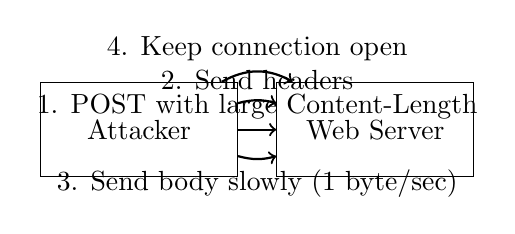
\begin{tikzpicture}[
    node distance=3cm,
    box/.style={rectangle,draw,minimum width=2.5cm,minimum height=1.2cm,align=center},
    arrow/.style={->,thick}
]
    \node[box] (attacker) {Attacker};
    \node[box,right of=attacker] (server) {Web Server};
    
    \draw[arrow] (attacker) -- node[above,sloped] {1. POST with large Content-Length} (server);
    \draw[arrow] (attacker) to[bend left=15] node[above,sloped] {2. Send headers} (server);
    \draw[arrow] (attacker) to[bend right=15] node[below,sloped] {3. Send body slowly (1 byte/sec)} (server);
    \draw[arrow] (attacker) to[bend left=30] node[above,sloped] {4. Keep connection open} (server);
\end{tikzpicture}
\caption{Slow POST Attack Flow}
\label{fig:slowpost}
\end{figure}

\subsection{HAProxy Protection Mechanisms}

\subsubsection{What is HAProxy?}
HAProxy (High Availability Proxy) is a free, very fast and reliable solution offering high availability, load balancing, and proxying for TCP and HTTP-based applications. It is particularly suited for web sites crawling under very high load while needing persistence or Layer 7 processing. HAProxy runs on event-driven, non-blocking engine, making it very efficient and suitable for high-traffic web sites.

Key features of HAProxy include:
\begin{itemize}
    \item \textbf{Load Balancing}: Distributes incoming requests across multiple backend servers
    \item \textbf{Health Checking}: Monitors backend server health and automatically removes failed servers
    \item \textbf{SSL Termination}: Handles SSL/TLS encryption and decryption
    \item \textbf{Rate Limiting}: Controls request rates to prevent abuse
    \item \textbf{Stick Tables}: Tracks client behavior for advanced traffic management
    \item \textbf{ACLs}: Access Control Lists for making routing decisions based on various criteria
\end{itemize}

\subsubsection{Stick Tables}
Stick tables are HAProxy's mechanism for tracking client behavior across multiple connections. They act as in-memory databases that store information about clients (typically identified by IP address) and their associated metrics.

\textbf{Key Concepts:}
\begin{itemize}
    \item \textbf{Type}: IP-based tracking (can also track other identifiers like user-agent, cookie, etc.)
    \item \textbf{Size}: Configurable table size (e.g., 100k entries) - when full, oldest entries are evicted
    \item \textbf{Expiration}: Automatic cleanup after specified time (e.g., 10 minutes)
    \item \textbf{Storage}: Various metrics like connection rate, request rate, bytes transferred, etc.
\end{itemize}

\textbf{Common Stick Table Store Options:}
\begin{itemize}
    \item \texttt{conn\_rate(10s)}: Number of connections per 10 seconds
    \item \texttt{req\_rate(10s)}: Number of requests per 10 seconds
    \item \texttt{bytes\_in\_rate(10s)}: Bytes received per 10 seconds
    \item \texttt{bytes\_out\_rate(10s)}: Bytes sent per 10 seconds
\end{itemize}

\textbf{Example Configuration:}
\begin{lstlisting}[language=bash]
# Define a stick table for tracking abusive IPs
backend abuse_tracker
    stick-table type ip size 100k expire 10m store conn_rate(10s)
\end{lstlisting}

\subsubsection{Access Control Lists (ACLs)}
Access Control Lists (ACLs) are HAProxy's primary mechanism for making routing decisions based on various conditions. ACLs evaluate to true or false and can be combined using logical operators.

\textbf{Common ACL Types:}
\begin{itemize}
    \item \textbf{Path-based ACLs}: Match URL paths (e.g., \texttt{path\_beg /bypass})
    \item \textbf{IP-based ACLs}: Match source IP addresses (e.g., \texttt{src 192.168.1.0/24})
    \item \textbf{Rate-based ACLs}: Match based on stick table data (e.g., \texttt{src\_conn\_rate(abuse\_tracker) gt 20})
    \item \textbf{Header-based ACLs}: Match HTTP headers (e.g., \texttt{hdr(User-Agent) -i bot})
    \item \textbf{Method-based ACLs}: Match HTTP methods (e.g., \texttt{method POST})
\end{itemize}

\textbf{ACL Usage Examples:}
\begin{lstlisting}[language=bash]
# Define ACLs
acl is_bypass path_beg /bypass
acl abusive_ip src_conn_rate(abuse_tracker) gt 20

# Use ACLs in routing decisions
use_backend direct_backend if is_bypass
use_backend reserve_backend if !abusive_ip
use_backend main_backend if abusive_ip
\end{lstlisting}

\textbf{ACL Operators:}
\begin{itemize}
    \item \texttt{eq}: Equal to
    \item \texttt{gt}: Greater than
    \item \texttt{lt}: Less than
    \item \texttt{beg}: Begins with
    \item \texttt{end}: Ends with
    \item \texttt{sub}: Contains substring
    \item \texttt{reg}: Regular expression match
\end{itemize}

\subsubsection{Integration of Stick Tables and ACLs}
The power of HAProxy's protection mechanisms comes from combining stick tables and ACLs:

\begin{enumerate}
    \item \textbf{Tracking}: Stick tables track client behavior (e.g., connection rates)
    \item \textbf{Evaluation}: ACLs evaluate conditions based on stick table data
    \item \textbf{Action}: Routing decisions are made based on ACL evaluation results
\end{enumerate}

\textbf{Complete Example:}
\begin{lstlisting}[language=bash]
# 1. Define stick table for tracking
backend abuse_tracker
    stick-table type ip size 100k expire 10m store conn_rate(10s)

# 2. Track connections in frontend
frontend http-in
    bind *:8081
    
    # Track client IP in stick table
    tcp-request connection track-sc0 src table abuse_tracker
    
    # Define ACL for abusive behavior
    acl abusive_ip src_conn_rate(abuse_tracker) gt 20
    
    # Route based on ACL evaluation
    use_backend reserve_backend if !abusive_ip
    use_backend main_backend if abusive_ip
\end{lstlisting}

This integration allows HAProxy to:
\begin{itemize}
    \item Dynamically identify abusive clients based on their behavior
    \item Route traffic to different backends based on client reputation
    \item Maintain service quality for legitimate users while handling attacks
    \item Automatically adapt to changing attack patterns
\end{itemize}

\section{Lab Setup}

\subsection{Environment Preparation}

\subsubsection{Step 1: Clone and Navigate}
\begin{lstlisting}[language=bash]
# Navigate to the lab directory
cd seed-proxy-lab

# Verify the structure
ls -la
\end{lstlisting}

\subsubsection{Step 2: Build and Start Containers}
\begin{lstlisting}[language=bash]
# Build and start all services
docker-compose up -d --build

# Verify all containers are running
docker-compose ps
\end{lstlisting}

\subsubsection{Step 3: Verify Services}
\begin{lstlisting}[language=bash]
# Check if nginx is accessible directly
curl http://localhost:8080

# Check if HAProxy is accessible
curl http://localhost:8081
\end{lstlisting}

\subsection{Network Topology}

\begin{figure}[H]
\centering
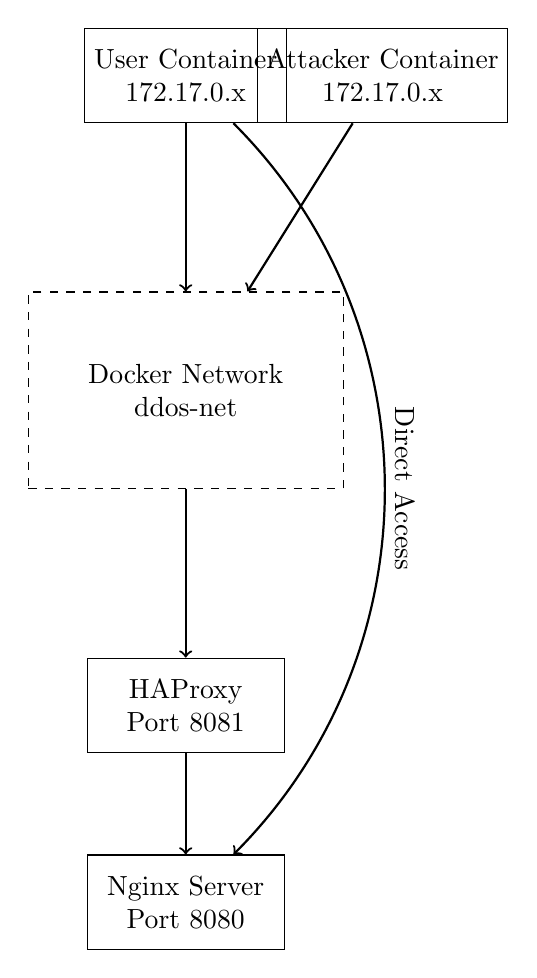
\begin{tikzpicture}[
    node distance=2.5cm,
    box/.style={rectangle,draw,minimum width=2.5cm,minimum height=1.2cm,align=center},
    arrow/.style={->,thick},
    network/.style={rectangle,draw,dashed,minimum width=4cm,minimum height=2.5cm,align=center}
]
    \node[box] (user) {User Container\\172.17.0.x};
    \node[box,right of=user] (attacker) {Attacker Container\\172.17.0.x};
    
    \node[network,below of=user,yshift=-1.5cm] (network) {Docker Network\\ddos-net};
    
    \node[box,below of=network,yshift=-1.5cm] (haproxy) {HAProxy\\Port 8081};
    \node[box,below of=haproxy] (nginx) {Nginx Server\\Port 8080};
    
    \draw[arrow] (user) -- (network);
    \draw[arrow] (attacker) -- (network);
    \draw[arrow] (network) -- (haproxy);
    \draw[arrow] (haproxy) -- (nginx);
    
    \draw[arrow] (user) to[bend left=45] node[above,sloped] {Direct Access} (nginx);
\end{tikzpicture}
\caption{Lab Network Topology}
\label{fig:topology}
\end{figure}

\section{Implementation Tasks}

\subsection{Task 1: HAProxy Configuration Implementation}

In this task, you will implement two key components of the HAProxy configuration. Open the file \texttt{seed-proxy-lab/haproxy/haproxy.cfg} and complete the following tasks:

\subsubsection{Task 1.1: Define Stick Table}
Complete the stick table configuration in the \texttt{abuse\_tracker} backend:

\begin{lstlisting}[language=bash, caption=HAProxy Configuration - Task 1.1]
# TODO: Task 1 - Define stick table for tracking abusive IPs
# Complete the stick table configuration below:
# - Type should be 'ip' for IP-based tracking
# - Size should be 100k entries
# - Expire after 10 minutes
# - Store connection rate over 10 seconds
backend abuse_tracker
    # ** FILL HERE **
    # stick-table type ip size 100k expire 10m store conn_rate(10s)
\end{lstlisting}

\textbf{Requirements:}
\begin{itemize}
    \item Type: \texttt{ip} for IP-based tracking
    \item Size: \texttt{100k} entries
    \item Expiration: \texttt{10m} (10 minutes)
    \item Storage: \texttt{conn\_rate(10s)} (connection rate over 10 seconds)
\end{itemize}

\subsubsection{Task 1.2: Define ACL for Abusive IPs}
Create ACL to identify abusive IPs:

\begin{lstlisting}[language=bash, caption=HAProxy Configuration - Task 1.2]
# TODO: Task 2 - Define ACL for abusive IPs
# Create an ACL that identifies IPs with more than 20 connections in 10 seconds
# ** FILL HERE **
# acl abusive_ip src_conn_rate(abuse_tracker) gt 20
\end{lstlisting}

\textbf{Requirements:}
\begin{itemize}
    \item Create ACL named \texttt{abusive\_ip}
    \item Check if connection rate from stick table is greater than 20
    \item Use \texttt{src\_conn\_rate(abuse\_tracker) gt 20}
\end{itemize}

\subsection{Task 2: Attack Script Implementation}

In this task, you will implement two key components of the slow POST attack script. Open the file \texttt{seed-proxy-lab/attacker/slow\_post\_threads.py} and complete the following tasks:

\subsubsection{Task 2.1: Implement Target Selection}
Complete the target host and port selection logic:

\begin{lstlisting}[language=python, caption=Attack Script - Task 2.1]
# TODO: Task 1 - Implement target host and port selection
# Complete the logic to set the correct host and port based on the target argument
# - If target is "proxy", use "haproxy" as host and 8081 as port
# - If target is "direct", use "nginx-server" as host and 80 as port
# ** FILL HERE **
if target == "proxy":
    # ** FILL HERE **
    pass
else:
    # ** FILL HERE **
    pass
\end{lstlisting}

\textbf{Requirements:}
\begin{itemize}
    \item If \texttt{target} is \texttt{"proxy"}: set \texttt{host = "haproxy"} and \texttt{port = 8081}
    \item If \texttt{target} is \texttt{"direct"}: set \texttt{host = "nginx-server"} and \texttt{port = 80}
\end{itemize}

\subsubsection{Task 2.2: Implement Slow Data Transmission}
Complete the slow data transmission logic:

\begin{lstlisting}[language=python, caption=Attack Script - Task 2.2]
# TODO: Task 2 - Implement slow data transmission
# Send data slowly to keep the connection open
# Send one byte at a time with a 0.05 second delay between sends
# ** FILL HERE **
while True:
    # ** FILL HERE **
    pass
\end{lstlisting}

\textbf{Requirements:}
\begin{itemize}
    \item Send one byte (\texttt{b"A"}) at a time
    \item Sleep for 0.05 seconds between sends
    \item Continue indefinitely to keep connection open
\end{itemize}

\section{Phase 1: Direct DDoS Attack}

\subsection{Objective}
Demonstrate how slow HTTP/TCP attacks can overwhelm a backend server when no protection is in place.

\subsection{Task 1: Baseline Performance Test}

\subsubsection{Step 1: Access User Container}
\begin{lstlisting}[language=bash]
# Access the user container
docker exec -it user sh
\end{lstlisting}

\subsubsection{Step 2: Measure Normal Response Time}
\begin{lstlisting}[language=bash]
# Test normal response time using container name
time curl -s http://nginx-server:80 > /dev/null
\end{lstlisting}

\subsubsection{Step 3: Monitor Server Resources}
\begin{lstlisting}[language=bash]
# In another terminal, monitor nginx server
docker exec -it nginx-server bash

# Monitor system resources
htop
\end{lstlisting}

\subsection{Task 2: Execute Slow POST Threads Attack (Direct)}

\subsubsection{Step 1: Access Attacker Container}
\begin{lstlisting}[language=bash]
# Access the attacker container
docker exec -it attacker bash
\end{lstlisting}

\subsubsection{Step 2: Launch Direct Attack}
\begin{lstlisting}[language=bash]
# Navigate to the attack directory
cd /app

# Run slow POST threads attack directly against nginx-server
python3 slow_post_threads.py direct protected
\end{lstlisting}

\subsubsection{Step 3: Monitor Impact}
\begin{lstlisting}[language=bash]
# In the nginx container, monitor connections
watch -n 1 "netstat -an | grep :80 | wc -l"
\end{lstlisting}

\subsubsection{Step 4: Test Legitimate User Access}
\begin{lstlisting}[language=bash]
# In the user container, test access during attack
time curl -s http://nginx-server:80 > /dev/null
\end{lstlisting}

\subsection{Expected Results}
\begin{itemize}
    \item Server response times increase significantly
    \item Connection count rises rapidly
    \item Legitimate users experience timeouts
    \item Server may become unresponsive
\end{itemize}

\section{Phase 2: HAProxy Protection Implementation}

\subsection{Objective}
Implement HAProxy-based protection mechanisms to mitigate slow HTTP/TCP attacks while maintaining service availability for legitimate users.

\subsection{Task 1: Configure HAProxy Protection}

\subsubsection{Step 1: Review Current Configuration}
The HAProxy configuration includes several protection mechanisms:

\begin{lstlisting}[language=bash, caption=HAProxy Configuration]
# IP tracking table (stick table)
backend abuse_tracker
    stick-table type ip size 100k expire 10m store conn_rate(10s)

frontend http-in
    bind *:8081
    log global

    # 1. Bypass path routing (handled first)
    acl is_bypass path_beg /bypass
    use_backend direct_backend if is_bypass

    # 2. Track IP into stick-table
    tcp-request connection track-sc0 src table abuse_tracker

    # 3. ACL for abusive IPs
    acl abusive_ip src_conn_rate(abuse_tracker) gt 20

    # 4. Routing based on IP behavior
    use_backend reserve_backend if !abusive_ip
    use_backend main_backend if abusive_ip

backend reserve_backend
    timeout server 1s
    option http-server-close
    server nginx nginx-server:80 maxconn 200 check

backend main_backend
    timeout server 1s
    option http-server-close
    server nginx nginx-server:80 maxconn 800 check

backend direct_backend
    timeout server 1s
    option http-server-close
    server nginx nginx-server:80
\end{lstlisting}

\subsubsection{Step 2: Understand Protection Mechanisms}

\textbf{Path-based Bypass:}
\begin{itemize}
    \item Requests starting with `/bypass` go directly to `direct_backend`
    \item No rate limiting or protection applied
    \item Useful for testing and monitoring
\end{itemize}

\textbf{IP-based Throttling:}
\begin{itemize}
    \item Tracks connection rate per IP over 10-second windows
    \item IPs with >20 connections in 10s are marked as abusive
    \item Abusive IPs routed to `main_backend` (800 max connections)
    \item Clean IPs routed to `reserve_backend` (200 max connections)
\end{itemize}

\subsection{Task 2: Test HAProxy Bypass Path (Attack Succeeds)}

\subsubsection{Step 1: Access User Container}
\begin{lstlisting}[language=bash]
# Access the user container
docker exec -it user sh
\end{lstlisting}

\subsubsection{Step 2: Test Bypass Path}
\begin{lstlisting}[language=bash]
# Test bypass path using container name
curl -v http://haproxy:8081/bypass/test
\end{lstlisting}

\subsubsection{Step 3: Launch Attack Using Bypass Path}
\begin{lstlisting}[language=bash]
# In the attacker container, launch attack using bypass path
python3 slow_post_threads.py proxy bypass
\end{lstlisting}

\subsubsection{Step 4: Test Legitimate User Access During Bypass Attack}
\begin{lstlisting}[language=bash]
# In the user container, test access during bypass attack
time curl -s http://haproxy:8081/ > /dev/null
\end{lstlisting}

\subsection{Task 3: Test HAProxy Protected Path (Attack Fails)}

\subsubsection{Step 1: Launch Attack Using Protected Path}
\begin{lstlisting}[language=bash]
# In the attacker container, launch attack using protected path
python3 slow_post_threads.py proxy protected
\end{lstlisting}

\subsubsection{Step 2: Monitor Protection Effectiveness}
\begin{lstlisting}[language=bash]
# Monitor HAProxy logs
docker logs -f haproxy

# Check connection distribution
docker exec -it haproxy haproxy -c -f /usr/local/etc/haproxy/haproxy.cfg
\end{lstlisting}

\subsubsection{Step 3: Test Legitimate User Access During Protected Attack}
\begin{lstlisting}[language=bash]
# In the user container, test access during protected attack
time curl -s http://haproxy:8081/ > /dev/null
\end{lstlisting}

\subsection{Task 4: Compare Results}

\subsubsection{Step 1: Analyze Attack Effectiveness}
\begin{lstlisting}[language=bash]
# Monitor HAProxy logs for protection activity
docker logs -f haproxy | grep -E "(abusive_ip|reserve_backend|main_backend)"

# Check nginx server status during different attack modes
docker exec -it nginx-server netstat -an | grep :80 | wc -l
\end{lstlisting}

\subsection{Attack scenarios Overview}

\subsubsection{Direct Attack (Phase 1)}
\begin{itemize}
    \item \textbf{Target:} nginx-server directly
    \item \textbf{Method:} Slow POST threads with 5500 concurrent connections
    \item \textbf{Result:} Server becomes unresponsive, legitimate users cannot access
    \item \textbf{Impact:} Complete service disruption
\end{itemize}

\subsubsection{Bypass Attack (Phase 2)}
\begin{itemize}
    \item \textbf{Target:} HAProxy with bypass path (/bypass)
    \item \textbf{Method:} Slow POST threads using bypass route
    \item \textbf{Result:} Attack succeeds, server becomes unresponsive
    \item \textbf{Impact:} Service disruption despite HAProxy presence
\end{itemize}

\subsubsection{Protected Attack (Phase 2)}
\begin{itemize}
    \item \textbf{Target:} HAProxy with protected path (/)
    \item \textbf{Method:} Slow POST threads using protected route
    \item \textbf{Result:} Attack fails, legitimate users can still access service
    \item \textbf{Impact:} Service remains available for legitimate users
\end{itemize}

\section{Real-World Proxy Load Balancing Applications}

\subsection{Introduction}
The HAProxy-based protection mechanisms demonstrated in this lab are widely used in real-world production environments. Understanding how proxies and load balancers work in practice helps students appreciate the practical applications of the concepts learned.

\subsection{Common Use Cases}

\subsubsection{1. Web Application Load Balancing}
\begin{itemize}
    \item \textbf{Traffic Distribution:} Distribute incoming requests across multiple backend servers
    \item \textbf{Health Checking:} Monitor server health and automatically remove failed servers
    \item \textbf{Session Persistence:} Maintain user sessions across multiple requests
    \item \textbf{SSL Termination:} Handle SSL/TLS encryption at the proxy level
\end{itemize}

\subsubsection{2. DDoS Protection and Mitigation}
\begin{itemize}
    \item \textbf{Rate Limiting:} Prevent abuse by limiting requests per IP address
    \item \textbf{Traffic Filtering:} Block malicious traffic based on patterns and signatures
    \item \textbf{Geographic Distribution:} Route traffic based on geographic location
    \item \textbf{Traffic Shaping:} Prioritize legitimate traffic over attack traffic
\end{itemize}

\subsubsection{3. High Availability and Failover}
\begin{itemize}
    \item \textbf{Active-Passive:} Primary server with backup servers on standby
    \item \textbf{Active-Active:} Multiple servers handling traffic simultaneously
    \item \textbf{Automatic Failover:} Switch to backup servers when primary fails
    \item \textbf{Load Distribution:} Balance load across multiple data centers
\end{itemize}

\subsection{Conclusion}
The concepts learned in this lab provide a foundation for understanding real-world proxy and load balancing implementations. The HAProxy configuration and protection mechanisms demonstrated here are directly applicable to production environments, where they help ensure high availability, security, and performance for web applications and services.

\section{Testing Your Implementation}

\subsection{Step 1: Verify HAProxy Configuration}
\begin{lstlisting}[language=bash]
# Check HAProxy configuration syntax
docker exec -it haproxy haproxy -c -f /usr/local/etc/haproxy/haproxy.cfg

# If successful, restart HAProxy
docker-compose restart haproxy
\end{lstlisting}

\subsection{Step 2: Test Attack Script}
\begin{lstlisting}[language=bash]
# Access attacker container
docker exec -it attacker bash

# Test the attack script
python3 slow_post_threads.py proxy protected
\end{lstlisting}

\subsection{Step 3: Verify Protection}
\begin{lstlisting}[language=bash]
# Access user container
docker exec -it user sh

# Test legitimate access during attack
curl -s http://haproxy:8081/
\end{lstlisting}

\section{Evaluation Criteria}

\subsection{Implementation Tasks (60\%)}
\begin{itemize}
    \item \textbf{HAProxy Configuration (30\%)}: Correct implementation of stick table and ACL
    \item \textbf{Attack Script (30\%)}: Correct implementation of target selection and slow data transmission
\end{itemize}

\subsection{Testing and Validation (40\%)}
\begin{itemize}
    \item \textbf{Configuration Validation (20\%)}: HAProxy configuration compiles and runs without errors
    \item \textbf{Attack Effectiveness (20\%)}: Attack script successfully demonstrates DDoS and protection mechanisms
\end{itemize}

\section{Submission Requirements}

\subsection{Required Deliverables}
\begin{itemize}
    \item Completed \texttt{haproxy.cfg} file with all TODO tasks implemented
    \item Completed \texttt{slow\_post\_threads.py} file with all TODO tasks implemented
    \item Screenshots showing successful compilation and testing
    \item Brief report explaining your implementation choices
\end{itemize}

\subsection{Submission Format}
Submit the following files:
\begin{enumerate}
    \item \texttt{haproxy.cfg} - Your completed HAProxy configuration
    \item \texttt{slow\_post\_threads.py} - Your completed attack script
    \item \texttt{implementation\_report.pdf} - Brief report (1-2 pages) explaining your implementation
    \item Screenshots of successful testing (as separate image files)
\end{enumerate}

\section{References}

\begin{enumerate}
    \item HAProxy Documentation: \url{https://www.haproxy.org/download/2.6/doc/intro.txt}
    \item SEED Labs: \url{https://seedsecuritylabs.org}
    \item Slowloris Attack: \url{https://en.wikipedia.org/wiki/Slowloris_(computer_security)}
    \item DDoS Protection Strategies: \url{https://www.cloudflare.com/learning/ddos/}
\end{enumerate}

\end{document}
